\documentclass[../../main]{subfiles}

\begin{document}
\chapter{測度空間}

\section{イントロダクション}

\cref{chapter:hilbert_space},\cref{chapter:probability_space}では,関数空間での直交射影を積分に基づいて論じた.
関数空間でも直交射影を定義できる理由は,\(\Lebesgue{2}(\Omega)=\Set{f\given\int_\Omega\abs{f(x)}^2\intd{x}<+\infty}\)がヒルベルト空間,つまり,完備な内積空間だからである.
そして,\(\Lebesgue{2}(\Omega)\)の完備性には,積分がリーマン積分ではなくルベーグ積分であることが効いている.

また,確率変数の期待値はルベーグ積分で定義される.これは,ルベーグ積分を使うと関数の定義域をより自由に選べることの恩恵である.まとめると,ルベーグ積分はリーマン積分に次の2点で優る.
\begin{enumerate}
  \item 積分と極限の相性がよい.
  \item 関数の定義域が\(\numset{R}^n\)の部分集合でなくともよい.
\end{enumerate}

これらの強みは主に,ルベーグ積分では面積の測り方(測度)を自由に決められること,そして,測度の観点から区別できないものは同一視できることに由来する.そのため,ルベーグ積分の利点を享受するには
\begin{enumerate}
  \item 面積が定義される集合のあつまり(\impact{σ‐加法族})を用意する.
  \item 各集合に面積を割り当てる写像(\impact{測度})を用意する.
  \item 積分を定義できる関数(\impact{可測関数})を規定する.
\end{enumerate}
という,3つの段階を要する.本章では,この3段階をどう踏んでいけばよいのかを,かけ足で概観する.

\section{測度論の基本概念}

\subsection{σ‐加法族}

集合\(S\)の部分集合全体を,\(S\)の\termdef{べき集合}\index{べきしゅうごう@べき集合}\indexsymbol{\(\powerset{S}\)}(power set)という.
以後,\(S\)のべき集合を\(\powerset{S}\)と表す.

\begin{definition}{σ‐加法族}{sigma_algebra}\index{しぐまかほうぞく@σ‐加法族}
  \(\Omega\)を集合,\(\sigmaalg{F}\)を\(\powerset{\Omega}\)の部分集合とする.
  \(\sigmaalg{F}\)が\(\Omega\)上の\termdef{σ‐加法族}(σ‐algebra)であるとは,\(\sigmaalg{F}\)が以下の条件を満たすことをいう.
  \begin{enumerate}
    \item \(\Omega\in\sigmaalg{F}\)である.
    \item 任意の\(A\in\sigmaalg{F}\)に対して\(\scomp{A}=\Omega\setminus A\in\sigmaalg{F}\)である.
    \item 任意の\(A_1,A_2,\dotsc\in\sigmaalg{F}\)に対して\(\bigcup_{n\in\numset{N}}A_n\in\sigmaalg{F}\)である.
  \end{enumerate}
\end{definition}

組\((\Omega,\sigmaalg{F})\)を\termdef{可測空間}\index{かそくくうかん@可測空間}(measurable space)という.

\begin{example}
  \(\Set{\emptyset,\Omega}\)と\(\powerset{\Omega}\)は\(\Omega\)上のσ‐加法族である.
\end{example}

\begin{example}\label{example:dice}
  \(\Omega=\Set{\dicei,\diceii,\diceiii,\diceiv,\dicev,\dicevi}\)を6元集合とし,\(O=\Set{\dicei,\diceiii,\dicev}\)とおく.
  このとき,\(\sigmaalg{G}=\Set{\emptyset,O,\scomp{O},\Omega}\)は\(\Omega\)上のσ‐加法族である.
\end{example}

\begin{definition}{生成するσ‐加法族}{}\index{せいせい@生成!しぐまかほうぞく@σ‐加法族}\index{しぐまかほうぞく@σ‐加法族!せいせいする@生成する\texttwoemdash}\indexsymbol{\(\sigmagen{\symcal{S}}\)}
  \(\Omega\)を集合,\(\symcal{S}\)を\(\powerset{\Omega}\)の部分集合とする.また,\(\symcal{S}\)を包含する\(\Omega\)上のσ‐加法族全体を\(\Sigma(\symcal{S})\)とおく.このとき,集合
  \[
    \sigmagen{\symcal{S}} = \bigcap_{\sigmaalg{F}\in\Sigma(\symcal{S})}\sigmaalg{F}
    = \Set{A\in\powerset{\Omega}\given\text{\(\Sigma(\symcal{S})\)の元すべてに\(A\)は属する}}
  \]
  は\(\Sigma(\symcal{S})\)に属する.\(\sigmagen{\symcal{S}}\)を\(\symcal{S}\)が\termdef{生成するσ‐加法族}(generated σ‐algebra)という.
\end{definition}

\begin{example}[ボレル集合族]\index{ぼれるしゅうごうぞく@ボレル集合族}\index{BR@\(\borelset{\numset{R}}\)}
  集合\(\symcal{S}=\Set{\ocival{-\infty}{a}\given a\in\numset{R}}\)により生成されるσ‐加法族を\(\numset{R}\)上の\termdef{ボレル集合族}(Borel algebra)といい,\(\borelset{\numset{R}}\)と表記する.
\end{example}

\begin{note}
  \(\borelset{\numset{R}}\)は\(\numset{R}\)の開集合系が生成するσ‐加法族でもある.実はより一般に,位相空間の開集合系が生成するσ‐加法族のことをボレル集合族という.
\end{note}

\begin{example}
  \cref{example:dice}のσ‐加法族\(\sigmaalg{G}\)は\(\sigmaalg{G}=\sigmagen{\Set{O}}\)と書ける.
  実際,\(\sigmaalg{F}\)が\(\Set{O}\)を包含するσ‐加法族なら\(\scomp{O}\in\sigmaalg{F}\),\(\sigmaalg{G}\subset\sigmaalg{F}\)である.
  つまり,\(\sigmaalg{G}\)は\(\Set{O}\)を包含する最小のσ‐加法族だから,\(\sigmaalg{G}=\sigmagen{\Set{O}}\)である.
\end{example}

\subsection{ボレル測度とルベーグ測度}

\begin{definition}{拡大実数}{extended_real}\index{かくだいじっすう@拡大実数}\index{R@\(\extendedreal\)}
  \(\numset{R}\)に正負の無限大\(+\infty,-\infty\notin\numset{R}\)を加えた集合\(\extendedreal=\numset{R}\cup\Set{\pm\infty}\)を\termdef{拡大実数}(extended real number)という.
  各\(a\in\numset{R}\),\(x\in\extendedreal\)に対し,\(\pm\infty\)との演算を以下の通り定義する(複合同順).
  \begin{gather*}
    a+(\pm\infty) = (\pm\infty)+a = \pm\infty,
    \quad a-(\pm\infty) = \mp\infty, \\
    (\pm\infty)+(\pm\infty) = \pm\infty,
    \quad(\pm\infty)-(\mp\infty) = \pm\infty, \\
    \frac{a}{\pm\infty} = 0,
    \quad x\cdot(\pm\infty) = (\pm\infty)\cdot x = \begin{cases}\pm\infty & (x>0),\\ 0 & (x=0), \\ \mp\infty & (x<0)\end{cases}
  \end{gather*}
\end{definition}

\begin{note}
  \((\pm\infty)+(\mp\infty)\)や\((\pm\infty)-(\pm\infty)\)などは定義されない.要するに,\(\extendedreal\)上では不定形でない極限のみ計算できる.また,普通\(0\cdot(\pm\infty)\)は不定形だが,ここでは\(0\cdot(\pm\infty)=0\)と定義した.
\end{note}

\(\seq{A_n}_{n\in\numset{N}}\)を集合列とする.\(\seq{A_n}_{n\in\numset{N}}\)が\termdef{互いに素}\index{たがいにそ@互いに素}(disjoint)であるとは,
異なる任意の2数\(i,j\in\numset{N}\)に対して\(A_i\cap A_j=\emptyset\)であることをいう.
互いに素な集合の和であることを強調したいときは,和集合\(\bigcup_nA_n\)を\(\bigsqcup_nA_n\)とも書く\indexsymbol{\(A\sqcup B\)}.

\begin{definition}{測度}{measure}\index{そくど@測度}\index{そくど@測度}
  \(\sigmaalg{F}\)をσ‐加法族とする.写像\(\mu\colon\sigmaalg{F}\to\ccival{0}{+\infty}\)が\(\sigmaalg{F}\)上の\termdef{測度}(measure)であるとは,
  \(\mu\)が以下の条件を満たすことをいう.
  \begin{enumerate}
    \item \(\mu(\emptyset)=0\)である.
    \item \(\sigmaalg{F}\)上の集合列\(\seq{A_n}_{n\in\numset{N}}\)が互いに素ならば\(\mu(\bigsqcup_{n\in\numset{N}}A_n)=\sum_{n=1}^\infty\mu(A_n)\)である.
  \end{enumerate}
\end{definition}

3つ組\((\Omega,\sigmaalg{F},\mu)\)を\termdef{測度空間}\index{そくどくうかん@測度空間}(measure space)という.
特に\(\mu(\Omega)=1\)であるとき,\(\mu\)を\termdef{確率測度}\index{かくりつそくど@確率測度}\index{そくど@測度!かくりつ@確率\texttwoemdash}(probability measure),\((\Omega,\sigmaalg{F},\mu)\)を\termdef{確率空間}\index{かくりつくうかん@確率空間}(probability space)という.
また,確率空間の\(\Omega\)に属する各元は\termdef{根源事象}\index{こんげんじしょう@根源事象}(elementary event),\(\sigmaalg{F}\)に属する各元は\termdef{事象}\index{じしょう@事象}(event)と呼ばれる.

\begin{example}[計数測度]\index{けいすうそくど@計数測度}\index{そくど@測度!けいすう@計数\texttwoemdash}
  \(\sigmaalg{F}\)をσ‐加法族とする.各\(A\in\sigmaalg{F}\)に対して,\(A\)が有限集合なら\(\mu(A)=\sizeof{A}\),無限集合なら\(\mu(A)=+\infty\)とすると,\(\mu\)は\(\sigmaalg{F}\)上の測度になる.
  \(\mu\)を\termdef{計数測度}(counting measure)という.
\end{example}

\begin{example}[ディラック測度]\index{でぃらっくそくど@ディラック測度}\index{そくど@測度!でぃらっく@ディラック\texttwoemdash}
  \((\Omega,\sigmaalg{F})\)を可測空間とし,\(x\in\Omega\)を1つ選ぶ.各\(A\in\sigmaalg{F}\)に対して,\(x\in A\)なら\(\delta_x(A)=1\),\(x\notin A\)なら\(\delta_x(A)=0\)とすると,\(\delta_x\)は\(\sigmaalg{F}\)上の測度になる.
  \(\delta_x\)を\termdef{ディラック測度}(Dirac measure)という.
\end{example}

\begin{example}\label{example:equally_possible}
  \(\Omega\)を\cref{example:dice}と同じにし,\(\sigmaalg{F}=\powerset{\Omega}\)とする.このとき,写像\(\prob\colon\sigmaalg{F}\to\ccival{0}{1}\),\(\prob(A)=(1/6)\sizeof{A}\)は\(\sigmaalg{F}\)上の確率測度である.
  \(\prob\)は「どの目が出るのも同様に確からしい(公平な)6面ダイスに関する確率」を表すと解釈できる.たとえば,奇数の目が出る確率は\(\prob(O)=1/2\)である.
\end{example}

\cref{example:equally_possible}のように\(\Omega\)が有限集合のときは,各\(\omega\in\Omega\)に対して\(\mu(\Set{\omega})\)の値を決定することで,測度\(\mu\)を直に構成できる.
しかし,たとえば\(\sigmaalg{B}(\numset{R})\)上の測度を定める場合,この方法は使えない.そうした状況では,σ‐加法族よりも考えやすい集合族の上で測度の雛形を作り,それをσ‐加法族全体へと拡張する.

\begin{definition}{有限加法族}{finite_additive_class}\index{ゆうげんかほうぞく@有限加法族}
  \(\Omega\)を集合,\(\sigmaalg{A}\)を\(\powerset{\Omega}\)の部分集合とする.
  \(\sigmaalg{A}\)が\(\Omega\)上の\termdef{有限加法族}(finitely additive class)であるとは,\(\sigmaalg{A}\)が以下の条件を満たすことをいう.
  \begin{enumerate}
    \item \(\Omega\in\sigmaalg{A}\)である.
    \item 任意の\(A\in\sigmaalg{A}\)に対して\(\scomp{A}=\Omega\setminus A\in\sigmaalg{A}\)である.
    \item 任意の\(A,B\in\sigmaalg{A}\)に対して\(A\cup B\in\sigmaalg{A}\)である.
  \end{enumerate}
\end{definition}

\begin{definition}{有限加法的測度}{finitely_additive_measure}\index{ゆうげんかほうてきそくど@有限加法的測度}\index{そくど@測度!ゆうげんかほうてき@有限加法的\texttwoemdash}
  \(\sigmaalg{A}\)を有限加法族とする.写像\(m\colon\sigmaalg{A}\to\ccival{0}{+\infty}\)が\(\sigmaalg{A}\)上の\termdef{有限加法的測度}(finitely additive measure)であるとは,
  \(m\)が以下の条件を満たすことをいう.
  \begin{enumerate}
    \item \(m(\emptyset)=0\)である.
    \item \(A,B\in\sigmaalg{A}\)が\(A\cap B=\emptyset\)を満たすとき,\(m(A\sqcup B)=m(A)+m(B)\)である.
  \end{enumerate}
\end{definition}

\begin{note}
  infiniteは「インフィニット」と読むが,finiteは「ファイナイト」と読む.
\end{note}

\begin{theorem}{ホップの拡張定理}{hopf_extension}\index{ほっぷのかくちょうていり@ホップの拡張定理}
  \(\sigmaalg{A}\)を集合\(\Omega\)上の有限加法族,\(m\)を\(\sigmaalg{A}\)上の有限加法的測度とする.このとき,以下の命題は同値である.
  \begin{enumerate}
    \item \(\sigmaalg{A}\)上の集合列\(\seq{A_n}_{n\in\numset{N}}\)が互いに素で\(\bigsqcup_{n\in\numset{N}}A_n\in\sigmaalg{A}\)を満たすとき,\(m(\bigsqcup_{n\in\numset{N}}A_n)=\sum_{n=1}^\infty m(A_n)\)である.
    \item \(\sigmagen{\sigmaalg{A}}\)上の測度\(\mu\)で,任意の\(A\in\sigmaalg{A}\)に対して\(\mu(A)=m(A)\)を満たすものが存在する.
  \end{enumerate}
  さらに,\(\sigmaalg{A}\)上の集合列\(\seq{A_n}_{n\in\numset{N}}\)で\(m(A_n)<+\infty\),\(\bigcup_{n\in\numset{N}}A_n=\Omega\)を満たすものが存在するとき,\(\mu\)は一意である.
  これを\termdef{ホップの拡張定理}(Hopf extension theorem)という.
\end{theorem}

\begin{proof}
各\(S\in\powerset{\Omega}\)に対し,\(\sigmaalg{A}\)上の集合列\(\seq{A_n}_{n\in\numset{N}}\)で\(S\subset\bigcup_{n\in\numset{N}}A_n\)を満たすもの全体を\(\operatornamewithlimits{cover}_{\sigmaalg{A}}S\)とおく.
そして,写像\(\mu^{\mathord{\ast}}\colon\powerset{\Omega}\to\ccival{0}{+\infty}\)を
\[
  \mu^{\mathord{\ast}}(S) = \inf\Set*{\sum_{n=1}^\infty m(A_n)\given\seq{A_n}_{n\in\numset{N}}\in\operatornamewithlimits{cover}_{\sigmaalg{A}}S}
\]
で定義する.すると,集合
\begin{equation}
  \label{equation:caratheodory_measurable}
  \Set{A\in\powerset{\Omega}\given\text{任意の\(E\in\powerset{\Omega}\)に対し\(\mu^{\mathord{\ast}}(A)=\mu^{\mathord{\ast}}(A\cap E)+\mu^{\mathord{\ast}}(A\setminus E)\)}}
\end{equation}
は完全加法族であり,\(\sigmaalg{A}\)を包含する.この集合を\(\sigmaalg{F}\)とおくと,\(\mu^{\mathord{\ast}}\)の始域を\(\sigmaalg{F}\)へと制限した写像\(\bar{\mu}\)は,\(\sigmaalg{F}\)上の測度であることが示せる.
したがって,\(\bar{\mu}\)の\(\sigmagen{\sigmaalg{A}}\)への制限\(\mu\)は\(\sigmagen{\sigmaalg{A}}\)上の測度である.
\end{proof}

\begin{note}
  \(\sigmaalg{A}\)上の集合列\(\seq{A_n}_{n\in\numset{N}}\)で\(m(A_n)<+\infty\),\(\bigcup_{n\in\numset{N}}A_n=\Omega\)を満たすものが存在するとき,\(m\)は\termdef{σ‐有限}\index{しぐまゆうげん@σ‐有限}(σ‐finite)であるという.
  本書が扱う(有限加法的)測度はすべてσ‐有限なので,\cref{theorem:hopf_extension}から定まる拡張された測度は常に一意である.
  また,集合\(A\subset\Omega\)が\cref{equation:caratheodory_measurable}の\(\sigmaalg{F}\)に属する\texttwoemdash つまり,任意の\(E\in\powerset{\Omega}\)に対して\(\mu^{\mathord{\ast}}(A)=\mu^{\mathord{\ast}}(A\cap E)+\mu^{\mathord{\ast}}(A\setminus E)\)である\texttwoemdash とき,
  \(A\)は\(\mu^{\mathord{\ast}}\)に関して\termdef{カラテオドリ可測}\index{からておどりかそく@カラテオドリ可測}(Carathéodory‐measurable)であるという.
\end{note}

\(\symcal{E}\)を左半開区間\(\ocival{a}{b}\cap\numset{R}\)(\(-\infty\leq a<b\leq+\infty\))の全体集合とすると,集合\(\sigmaalg{A}=\Set{\emptyset}\cup\Set{\bigsqcup_{k=1}^nI_k\given\text{\(I_1,\dots,I_n\in\symcal{E}\)は互いに素}}\)は有限加法族をなし,
\(\sigmagen{\sigmaalg{A}}=\borelset{\numset{R}}\)が成り立つ.\(\sigmaalg{A}\)上の有限加法的測度\(\operatorname{vol}\)を
\[
  \operatorname{vol}\pqty*{\bigsqcup_{k=1}^n\ocival{a_k}{b_k}} = \sum_{k=1}^n(b_k-a_k)
\]
で定義する.このとき\(\operatorname{vol}\)はσ‐有限かつ\nameref{theorem:hopf_extension}の条件を満たすので,\(\borelset{\numset{R}}\)上の測度\(\mu\)へと一意に拡張できる.
この\(\borelset{\numset{R}}\)上の測度\(\mu\)を\termdef{ボレル測度}\index{ぼれるそくど@ボレル測度}\index{そくど@測度!ぼれる@ボレル\texttwoemdash}(Borel measure)という.
また,\(m=\operatorname{vol}\)のときの\(\bar{\mu}\)を\termdef{ルベーグ測度}\index{るべーぐそくど@ルベーグ測度}\index{そくど@測度!るべーぐ@ルベーグ\texttwoemdash}(Lebesgue measure)という.

\section{ルベーグ積分}

以下,\((\Omega,\sigmaalg{F},\mu)\)を測度空間とする.

\subsection{ルベーグ積分}

\begin{definition}{可測関数}{}\index{かそくかんすう@可測関数}
  関数\(f\colon\Omega\to\numset{R}\)が\termdef{可測関数}(\(\sigmaalg{F}\)‐可測,measurable function)であるとは,
  任意の\(A\in\borelset{\numset{R}}\)に対して\(\inv{f}{A}\in\sigmaalg{F}\)が成立することをいう.
\end{definition}

特に,確率空間における可測関数は(実数値)\termdef{確率変数}\index{かくりつへんすう@確率変数}(random variable)とも呼ばれる.

\begin{proposition}{}{sigmagen_and_measurable}
  集合\(\symcal{S}\subset\powerset{\numset{R}}\)が\(\sigmagen{\symcal{S}}=\borelset{\numset{R}}\)を満たすとき,任意の\(A\in\symcal{S}\)に対して\(\inv{f}{A}\in\sigmaalg{F}\)が成立すれば,\(f\)は可測関数である.
  特に,任意の\(a\in\numset{R}\)に対して\(\inv{f}{\ocival{-\infty}{a}}\in\sigmaalg{F}\)なら,\(f\)は可測関数である.
\end{proposition}

\begin{proof}
  集合\(\sigmaalg{G}=\Set{A\in\powerset{\numset{R}}\given\inv{f}{A}\in\sigmaalg{F}}\)はσ‐加法族であり,仮定から\(\symcal{S}\subset\sigmaalg{G}\)なので\(\sigmagen{\symcal{S}}\subset\sigmaalg{G}\)である.よって,\(f\)は可測関数である.
\end{proof}

\begin{definition}{単関数}{}\index{しじかんすう@指示関数}\index{たんかんすう@単関数}\indexsymbol{\(\indicator_A\)}
  \(a_1,\dots,a_n\in\numset{R}\)と互いに素な\(A_1,\dots,A_n\in\sigmaalg{F}\)により,
  次の形で表せる関数\(\phi\colon\Omega\to\numset{R}\)を\termdef{単関数}(simple function)という.
  \[
    \phi(x) = \sum_{k=1}^na_k\indicator_{A_k}(x),
    \quad\indicator_{A_k}(x) = \begin{cases}1 & (x\in A_k),\\ 0 & (x\notin A_k)\end{cases}
  \]
\end{definition}

非負値単関数\(\phi=\sum_{k=1}^na_k\indicator_{A_k}\)については,積分\(\int\phi\measured{\mu}=\int\phi(x)\measured[x]{\mu}\)を
\[
  \int\phi\measured{\mu} = \sum_{k=1}^na_k\mu(A_k)
\]
で定義できる.このことを利用して,非負値可測関数\(f\)の積分を
\[
  \int f\measured{\mu} = \sup\Set*{\int\phi\measured{\mu}\given\text{\(\phi\in\simplefuncs{\sigmaalg{F}}\),\(0\leq\phi\leq f\)}}
\]
で定義する.ただし,\(\simplefuncs{\sigmaalg{F}}\)は単関数の全体集合であり,\(\phi\leq f\)は任意の\(x\in\Omega\)に対し\(\phi(x)\leq f(x)\)であることを意味する.

\begin{figure}[htbp]
  \centering
  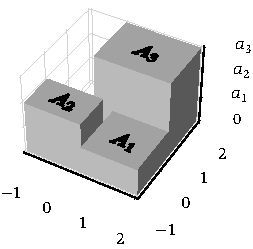
\includegraphics{figures/simple_function.pdf}
  \caption{\(\phi=a_1\indicator_{A_1}+a_2\indicator_{A_2}+a_3\indicator_{A_3}\)の模式図.}
\end{figure}

\begin{wrapfigure}[8]{o}{0pt}
  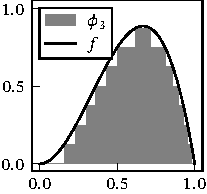
\includegraphics{figures/integration.pdf}
\end{wrapfigure}

より具体的に,\(\int f\measured{\mu}\)を非負値単関数の積分に関する極限で表すこともできる.\(\midx{E}{n}{k}=\inv{f}{\coival{2^{-n}k}{2^{-n}(k+1)}}\)とする.このとき
\[
  \phi_n = n\indicator_{\inv{f}{\coival{n}{+\infty}}}+\sum_{k=0}^{2^nn-1}\frac{k}{2^n}\indicator_{\midx{E}{n}{k}}
\]
は非負値単関数で,\(\int\phi_n\measured{\mu}\to\int f\measured{\mu}\)(\(n\to\infty\))である.

\(f\)が負の値をとりうる可測関数のときは,\(f^{\mathord{+}}(x)=\max\Set{f(x),0}\)と\(f^{\mathord{-}}(x)=\max\Set{-f(x),0}\)が非負値可測関数であることを利用して
\[
  \int f\measured{\mu} = \int f^{\mathord{+}}\measured{\mu}-\int f^{\mathord{-}}\measured{\mu}
\]
とする.ただし,\(\int f^{\mathord{-}}\measured{\mu}=\int f^{\mathord{+}}\measured{\mu}=+\infty\)のとき\(\int f\measured{\mu}\)は定義されない.
\(\int f^{\mathord{-}}\measured{\mu}\)と\(\int f^{\mathord{+}}\measured{\mu}\)がともに有限\texttwoemdash つまり\(\int\abs{f(x)}\measured[x]{\mu}<+\infty\)\texttwoemdash のとき,\(f\)は\termdef{可積分}\index{かせきぶん@可積分}(integrable)であるという.また,集合\(S\in\sigmaalg{F}\)上での積分は
\[
  \int_Sf\measured{\mu} = \int_Sf(x)\measured[x]{\mu}
  = \int f(x)\indicator_S(x)\measured[x]{\mu}
\]
で定義される.

特に\((\Omega,\sigmaalg{F},\prob)\)が確率空間のとき,\(\int X\measured{\prob}\)を確率変数\(X\)の\termdef{期待値}\index{きたいち@期待値}\index{E@\(\expval[X]\)}(expected value)といい,\(\expval[X]\)と書く.
また,\(\int_AX\measured{\prob}\)を\(\expval[X,A]\)\index{E@\(\expval[X,A]\)}とも表記する.

\begin{example}
  \cref{example:equally_possible}の確率空間\((\Omega,\sigmaalg{F},\prob)\)において,各\(\omega\in\Omega\)に対し\(X(\omega)\)を\(\omega\)の目で定義する.すなわち\(X(\dicei)=1\),\(X(\diceii)=2\)のようにする.
  このとき\(X=1\indicator_{\Set{\dicei}}+2\indicator_{\Set{\diceii}}+\dots+6\indicator_{\Set{\dicevi}}\)だから
  \[
    \expval[X] = 1\prob({\Set{\dicei}})+2\prob(\Set{\diceii})+\dots+6\prob({\Set{\dicevi}})
    = \frac{1+2+\dots+6}{6}
    = \frac{7}{2}
  \]
  であり,これは公平な6面ダイスの出目の期待値に相当する.
\end{example}

以上で定義した積分を\termdef{ルベーグ積分}\index{るべーぐせきぶん@ルベーグ積分}(Lebesgue integration)という.
ルベーグ積分とリーマン積分の間には,次の関係がある.

\begin{proposition}{}{}
  実数値関数\(f\)は有界閉区間\(\ccival{a}{b}\)上で定義され有界とする.このとき,\(f\)がリーマン積分できれば\(f\)はルベーグ測度に関して可積分で
  \[
    \int_a^bf(x)\intd{x} = \int_{\ccival{a}{b}}f(x)\measured[x]{\lambda}\quad\text{(\(\lambda\)は\(\numset{R}\)上のルベーグ測度)}
  \]
  が成立する.
\end{proposition}

\begin{note}\index{でぃりくれせきぶん@ディリクレ積分}
  積分区間が非有界なときは注意が要る.たとえば,\termdef{ディリクレ積分}(Dirichlet integral)
  \[
    \int_0^\infty\frac{\sin x}{x}\intd{x} = \lim_{\varepsilon\downarrow 0}\int_\varepsilon^1f(x)\intd{x}+\lim_{R\to\infty}\int_1^Rf(x)\intd{x}\quad(f(x)=(1/x)\sin x)
  \]
  の値は,広義積分の意味で\(\krez/2\)であることが知られている.しかし\(\int_{\ooival{0}{+\infty}}f^{\mathord{+}}\measured{\lambda}=\int_{\ooival{0}{+\infty}}f^{\mathord{-}}\measured{\lambda}=+\infty\)であり,ルベーグ積分できない.
\end{note}

最後に,複素数値可測関数の積分を定義しよう.関数\(\rpart f(x)\),\(\ipart f(x)\)がどちらも\(\sigmaalg{F}\)‐可測であるとき,関数\(f\colon\Omega\to\numset{C}\)は\(\sigmaalg{F}\)‐可測であるという.\(f\)の積分は
\[
  \int f\measured{\mu}=\int\rpart f(x)\measured[x]{\mu}+\iuni\int\ipart f(x)\measured[x]{\mu}
\]
で定義される.

\subsection{収束定理}

極限と積分を交換したいときは,以下の定理が非常に強力である.
\cref{theorem:monotone_convergence,theorem:fatou,theorem:dominated_convergence}はすべて,任意の測度空間\((\Omega,\sigmaalg{F},\mu)\)上で成立する.

\begin{theorem}{単調収束定理}{monotone_convergence}\index{たんちょうしゅうそくていり@単調収束定理}\index{MCT|see{単調収束定理}}
  可測関数列\(\seq{f_n}_{n\in\numset{N}}\)が\(0\leq f_1\leq f_2\leq\dotsb\)を満たすとき
  \[
    \lim_{n\to\infty}\int f_n(x)\measured[x]{\mu} = \int\pqty*{\lim_{n\to\infty}f_n(x)}\measured[x]{\mu}
  \]
  である.これを\termdef{単調収束定理}(monotone convergence theorem; MCT)という.
\end{theorem}

\begin{theorem}{ファトゥの補題}{fatou}\index{ふぁとうのほだい@ファトゥの補題}
  任意の可測関数列\(\seq{f_n}_{n\in\numset{N}}\)に対して
  \[
    \int\pqty*{\liminf_{n\to\infty}f_n(x)}\measured[x]{\mu} \leq \liminf_{n\to\infty}\int f_n(x)\measured[x]{\mu}
  \]
  である.これを\termdef{ファトゥの補題}(Fatou's lemma)という.
\end{theorem}

\begin{theorem}{優収束定理}{dominated_convergence}\index{ゆうしゅうそくていり@優収束定理}\index{DCT|see{優収束定理}}
  複素数値可測関数列\(\seq{f_n}_{n\in\numset{N}}\)が各点収束し,すべての\(n\in\numset{N}\),\(x\in\Omega\)で\(\abs{f_n(x)}\leq g(x)\)を満たす可積分関数\(g\)があれば
  \[
    \lim_{n\to\infty}\int f_n(x)\measured[x]{\mu} = \int\pqty*{\lim_{n\to\infty}f_n(x)}\measured[x]{\mu}
  \]
  である.これを\termdef{優収束定理}(dominated convergence theorem; DCT)という.
\end{theorem}

\section{確率論の基本概念}

本節では,確率空間\((\Omega,\sigmaalg{F},\prob)\)上で定義される諸概念を見ていく.

確率論ではしばしば,実数\(x\)に関する条件\(C(x)\)と確率変数\(X\)に対して,集合\(\Set{\omega\in\Omega\given C(X(\omega))}\)を\(\Set{C(X)}\)と書く.
たとえば\(\Set{X=1}=\Set{\omega\in\Omega\given X(\omega)=1}=\inv{X}{1}\),\(\prob(X=Y)=\prob(\Set{\omega\in\Omega\given X(\omega)=Y(\omega)})\)である.

\subsection{確率変数が定める量}

個々の確率変数の様子は,以下の関数から解析できる.

\begin{definition}{}{}\index{るいせきぶんぷかんすう@累積分布関数}\index{かくりつみつどかんすう@確率密度関数}\index{かくりつしつりょうかんすう@確率質量関数}\index{CDF|see{累積分布関数}}\index{PDF|see{確率密度関数}}\index{PMF|see{確率質量関数}}
  \(X\)を確率変数とする.
  \begin{enumerate}
    \item 関数\(F_X(x)=\prob(X\leq x)\)を\(X\)の\termdef{累積分布関数}(cumulative distribution function; CDF)という.
    \item 像\(\ran{X}{\Omega}\)が有限または可算集合のとき,関数\(p_X(x)=\prob(X=x)\)を\(X\)の\termdef{確率質量関数}(probability mass function; PMF)という.
    \item \(F_X\)が導関数\(f_X(x)=F_X'(x)\)を持つとき,\(f_X\)を\(X\)の\termdef{確率密度関数}(probability density function; PDF)という\footnotemark.
  \end{enumerate}
\end{definition}

\footnotetext{測度論を活用して,確率密度関数をより弱い仮定の下で定義することもできる\cite{funaki2022}.}
写像\(\imgmeasure{X}{\prob}\colon\borelset{\numset{R}}\to\ccival{0}{1}\)を\((\imgmeasure{X}{\prob})(A)=\prob(X\in A)\)で定義すると,\(\imgmeasure{X}{\prob}\)は\(\borelset{\numset{R}}\)上の確率測度になる.
\(\imgmeasure{X}{\prob}\)を\(X\)の\termdef{確率分布}\index{かくりつぶんぷ@確率分布}\index{P@\(\imgmeasure{X}{\prob}\)}(probability distribution),もしくは\(X\)による\(\prob\)の\termdef{像測度}\index{ぞうそくど@像測度}\index{そくど@測度!ぞう@像\texttwoemdash}(image measure)という.
\(X\)が確率質量関数\(p_X\)を持つとき,任意の\(A\in\borelset{\numset{R}}\)に対して
\[
  (\imgmeasure{X}{\prob})(A) = \sum_{x\in A}p_X(x)
\]
が成立する.同様に,\(X\)が確率密度関数\(f_X\)を持つとき
\[
  (\imgmeasure{X}{\prob})(A) = \int_Af_X(x)\measured[x]{\lambda}\quad\text{(\(\lambda\)は\(\numset{R}\)上のルベーグ測度)}
\]
が成立する.

これらの関数は,期待値を計算するとき重用される.\(\numset{R}\)上のボレル可測関数\(f\)に関して\(\expval[f(X)]=\int f(X(\omega))\measured[\omega]{\prob}\)だが,
この値を求めるには\(X(\omega)\to x\),\(1\measured[\omega]{\prob}\to f_X(x)\measured[x]{\lambda}\)と置き換えて,\(\int f(x)f_X(x)\measured[x]{\lambda}\)を計算すればよい.

\subsection{条件つき期待値}

\cref{example:dice,example:equally_possible}において,確率変数\(X\)の期待値は\(7/2\)であった.
これは,公平な6面ダイスをなんども投げ続けたとき,出目は平均的に\(7/2\)くらいの値をとることを意味する.
しかし,出目が奇数のとき,すなわち\(O\)に属するときだけ勘定に入れると条件づけた場合,\(X\)の期待値は変わると予想される.
直感的には,この条件の下で\(\dicei,\diceiii,\dicev\)が出る確率は等しく\(1/3\)であり,\(X\)の期待値は\((1+3+5)/3=3\)になるだろう.

以上の考え方に基づいて,事象\(A\)の下での事象\(B\)の\termdef{条件つき確率}\(\condprob{B\given A}\),確率変数\(X\)の\termdef{条件つき期待値}\(\condexpval{X\given A}\)を,それぞれ
\[
  \condprob{B\given A} = \frac{\prob(B\cap A)}{\prob(A)},
  \quad\condexpval{X\given A} = \frac{\expval[X,A]}{\prob(A)}
\]
と定義する(\(\prob(A)=0\)のときはどちらも定義しない).

出目の偶奇に関する事象全体は,σ‐加法族\(\sigmaalg{G}=\Set{\emptyset,O,\scomp{O},\Omega}\)である.\(\sigmaalg{G}\)‐可測な確率変数\(\condexpval{X\given\sigmaalg{G}}\)を
\begin{equation}
  \label{equation:discrete_conditional_expectation}
  \condexpval{X\given\sigmaalg{G}}(\omega) = \sum_{A\in\Set{O,\scomp{O}}}\condexpval{X\given A}\indicator_A(\omega)
  = \begin{cases}\condexpval{X\given O} & (\omega\in O),\\ \condexpval{X\given\scomp{O}} & (\omega\in\scomp{O})\end{cases}
\end{equation}
と定める.このとき,\(\condexpval{X\given\sigmaalg{G}}\)は各\(\omega\in\Omega\)に対し,\(\omega\)が属する\(\sigmaalg{G}\)上の事象で条件づけたときの,\(X\)の条件つき期待値を与える確率変数である.
確率変数\(\condexpval{X\given\sigmaalg{G}}\)をσ‐加法族\(\sigmaalg{G}\)の下での\(X\)の条件つき期待値という.
もう少し一般に,\(\sigmaalg{G}\)が\(\Omega\)の有限または可算な分割\(\Omega=\bigsqcup_{n\in I}A_n\)(\(A_n\in\sigmaalg{F}\),\(\prob(A_n)>0\))から生成される場合は,\(\condexpval{X\given\sigmaalg{G}}\)を\cref{equation:discrete_conditional_expectation}と同様に
\[
  \condexpval{X\given\sigmaalg{G}}(\omega) = \sum_{n\in I}\condexpval{X\given A_n}\indicator_{A_n}(\omega)\quad(\sigmaalg{G}=\sigmagen{\Set{A_n\given n\in I}})
\]
で定義できる.

以下では,一般のσ‐加法族\(\sigmaalg{G}\)に対して通用する\(\condexpval{X\given\sigmaalg{G}}\)の定義を考える.
\(X\)と\(Y\)を実数値確率変数とする.\(X\)と\(Y\)の値にはなんらかの関係があり,\(Y\)の値に関する条件の下で,\(X\)の期待値が持つ性質を解析したい.

\begin{note}
  たとえば,\(Y\)は気温,\(X\)はアイスクリームの売上と考えるとよい.  
\end{note}

\(Y\)の値に関する事象全体は,σ‐加法族\(\sigmaalg{G}=\Set{\inv{Y}{A}\given A\in\borelset{\numset{R}}}\)である.
また,\(y\fallingdotseq n\increment y\),\(0<\increment y\ll 1\)なら\(\condexpval{X\given\delta Y_n}\)(\(\delta Y_n=\Set{(n-1)\increment y<Y\leq n\increment y}\))はおおむね,条件\(Y=y\)の下での\(X\)の期待値を表すとみられる.

\(\Omega=\bigsqcup_{n\in\numset{Z}}\delta Y_n\)であるから,各\(\prob(\delta Y_n)\)の値が正なら\(\condexpval{X\given\sigmaalg{G}_{\increment y}}\)を
\[
  \condexpval{X\given\sigmaalg{G}_{\increment y}}(\omega) = \sum_{n\in\numset{Z}}\condexpval{X\given\delta Y_n}\indicator_{\delta Y_n}(\omega)\quad(\sigmaalg{G}_{\increment y}=\sigmagen{\Set{\delta Y_n\given n\in\numset{Z}}})
\]
と定義できる.\(\condexpval{X\given\sigmaalg{G}_{\increment y}}(\omega)\)の値は集合\(\Set{Y=y}\)上で一定であり,条件\(\delta Y_n\)(つまり\(Y\fallingdotseq y\))の下での\(X\)の期待値を表す.
そこで,いったん\(\condexpval{X\given\sigmaalg{G}}\)を
\[
  \condexpval{X\given\sigmaalg{G}}(\omega) \questeq \lim_{\increment y\to 0}\condexpval{X\given\sigmaalg{G}_{\increment y}}(\omega)
  = \lim_{\increment y\to 0}\sum_{n\in\numset{Z}}\condexpval{X\given\delta Y_n}\indicator_{\delta Y_n}(\omega)
\]
と「定義」してみよう.任意の\(B\in\borelset{\numset{R}}\)に対し,\(\expval\)と\(\lim\sum\)が交換できれば
\begin{align}
  \expval[\condexpval{X\given\sigmaalg{G}},Y\in B] &= \lim_{\increment y\to 0}\sum_{n\in\numset{Z}}\frac{\expval[X,\delta Y_n]}{\prob(\delta Y_n)}\expval[\indicator_{\delta Y_n},Y\in B] \\
  &= \lim_{\increment y\to 0}\sum_{n\in\numset{Z}}\expval[X,\delta Y_n]\frac{\prob(\Set{Y\in B}\cap\delta Y_n)}{\prob(\delta Y_n)} \\
  &= \lim_{\increment y\to 0}\sum_{n\in\numset{Z}}\expval[X,\delta Y_n]\condprob{Y\in B\given\delta Y_n} \label{equation:limit_of_conditional_expectation}
\end{align}
となる.事象\(\Set{Y=y}\)の下での\(\Set{Y\in B}\)の条件つき確率は,\(y\in B\)のとき\(1\),\(y\notin B\)のとき\(0\)と考えるのが妥当だろう.
つまり,大雑把に言って\cref{equation:limit_of_conditional_expectation}は,\(y\in B\)となるすべての\(y\in\numset{R}\)に関して\(\expval[X,Y=y]\)を足しているから
\[
  \expval[\condexpval{X\given\sigmaalg{G}},A] \questeq \expval[X,A]\quad(A=\Set{Y\in B})
\]
と考えられる.

実は逆に,\(\condexpval{X\given\sigmaalg{G}}\)は「任意の\(A\in\sigmaalg{G}\)に対し\(\expval[\condexpval{X\given\sigmaalg{G}},A]=\expval[X,A]\)を満たす」確率変数として定義される.

\begin{definition}{条件つき期待値}{conditional_expectation}\index{じょうけんつききたいち@条件つき期待値}\index{きたいち@期待値!じょうけんつき@条件つき\texttwoemdash}\index{らどんにこでぃむのていり@ラドン・ニコディムの定理}\index{E@\(\condexpval{X\given\sigmaalg{G}}\)}
  \((\Omega,\sigmaalg{F},\prob)\)は確率空間で,\(\Omega\)上のσ‐加法族\(\sigmaalg{G}\)は\(\sigmaalg{G}\subset\sigmaalg{F}\)を満たすとする.また,\(X\)は\((\Omega,\sigmaalg{F},\prob)\)上の確率変数とする.
  このとき,\(\sigmaalg{G}\)‐可測な確率変数\(Y\)で,任意の\(A\in\sigmaalg{G}\)に対し\(\expval[Y,A]=\expval[X,A]\)を満たすものが存在する\footnotemark .
  \(Y\)を\(\sigmaalg{G}\)の下での\(X\)の\termdef{条件つき期待値}(conditional expectation)といい,\(\condexpval{X\given\sigmaalg{G}}\)と書く.
\end{definition}
\footnotetext{これは\termdef{ラドン・ニコディムの定理}(Radon–Nikodým theorem)から保証される.}
\cref{definition:conditional_expectation}の\(\condexpval{X\given\sigmaalg{G}}\)は,測度\(0\)の集合上での違いを除いて一意に定まる.すなわち,\(\sigmaalg{G}\)‐可測な確率変数\(Y\)と\(Y'\)がともに\(\condexpval{X\given\sigmaalg{G}}\)の条件を満たすとき,\(\prob(Y\neq Y')=0\)である.
このことを\(Y=Y'\almostsurely\)\index{ほとんどかくじつに@ほとんど確実に}\index{as@a{.}s{.}}と表す\footnote{a{.}s{.}はalmost surely(ほとんど確実に)の略.}.

また,\(\indicator_A\)(\(A\in\sigmaalg{F}\))の条件つき期待値\(\condexpval{\indicator_A\given\sigmaalg{G}}\)を\(\sigmaalg{G}\)の下での\(A\)の\termdef{条件つき確率}\index{じょうけんつきかくりつ@条件つき確率}(conditional probability)といい,\(\condprob{A\given\sigmaalg{G}}\)\index{P@\(\condprob{A\given\sigmaalg{G}}\)}と書く.

\section{\texorpdfstring{\(\Lebesgue{p}\)空間}{Lp空間}}

以下,\((\Omega,\sigmaalg{F},\mu)\)を測度空間,\(\numset{K}\)を\(\numset{R}\)または\(\numset{C}\)とする.

\begin{definition}{零集合}{}\index{ぜろしゅうごう@零集合}
  \(A\)を\(\Omega\)の部分集合とする.\(\mu(N)=0\),\(A\subset N\)を満たす集合\(N\in\sigmaalg{F}\)があるとき,\(A\)は\termdef{\(\mu\)‐零集合}(\(\mu\)‐null set)であるという.
\end{definition}

\begin{definition}{ほとんどいたるところ}{}\index{ほとんどいたるところ}\index{ae@a{.}e{.}}
  \begin{enumerate}
    \item \(C(\omega)\)を\(\Omega\)の元\(\omega\)に関する条件とする.集合\(\scomp{\Set{\omega\given C(\omega)}}\)が\(\mu\)‐零集合であるとき,\(C(\omega)\)は\termdef{ほとんどいたるところ}(almost everywhere; a{.}e{.})成立するという.
      このことを\(C(\omega)\almosteverywhere[\mu][\omega\in\Omega]\)と書く.
    \item 関数\(f\colon\Omega\to\numset{K}\)は\(\sigmaalg{F}\)‐可測で,\(C(z)\)は\(\numset{K}\)の元\(z\)に関する条件とする.\(C(f(\omega))\almosteverywhere[\mu][\omega\in\Omega]\)であるとき,これを\(C(f)\almosteverywhere[\mu]\)と表す.
  \end{enumerate}
\end{definition}

\begin{note}
  すべての\(\mu\)‐零集合が\(\sigmaalg{F}\)に属するとき,\(\mu\)を\termdef{完備測度}\index{かんびそくど@完備測度}\index{そくど@測度!かんび@完備\texttwoemdash}(complete measure)という.
  \(\numset{R}\)上のボレル測度は完備測度でないが,ルベーグ測度は完備測度である.
\end{note}

\(1\leq p<+\infty\)とする.\cref{chapter:hilbert_space}で見たように,\(\int\abs{f(x)}^p\measured[x]{\mu}<+\infty\)を満たす可測関数\(f\colon\Omega\to\numset{K}\)からなる空間は,応用的にも非常に重要である.
この空間を\(\Lebesgue*{p}=\Lebesgue*{p}(\Omega,\sigmaalg{F},\mu)\)としよう.\(\Lpseminorm{p}{\holder}\)を
\[
  \Lpseminorm{p}{f} = \pqty*{\int\abs{f(x)}^p\measured[x]{\mu}}^{1/p}
\]
で定義すると,\termdef{ミンコフスキーの不等式}\index{みんこふすきーのふとうしき@ミンコフスキーの不等式}(Minkowski inequality)
\begin{equation}
  \label{equation:minkowski}
  \Lpseminorm{p}{f+g} \leq \Lpseminorm{p}{f}+\Lpseminorm{p}{g}
\end{equation}
から,\(\Lebesgue*{p}\)はベクトル空間である.また,\(\Lpseminorm{p}{\holder}\)はノルムの条件のうち\(\Lpseminorm{p}{af}=\abs{a}\Lpseminorm{p}{f}\),\(\Lpseminorm{p}{f+g}\leq\Lpseminorm{p}{f}+\Lpseminorm{p}{g}\)を満たす.

しかし厄介なことに,\(\Lpseminorm{p}{\holder}\)が任意の\(f\in\Lebesgue*{p}\)に対して\(\Lpseminorm{p}{f}=0\iff f=0\)を満たすのは,\(\mu\)が特殊な測度のときに限られる.一方で,次の事実がある.

\begin{proposition}{}{kernel_of_integration}
  \(f\)を可測関数とする.このとき,\(f\)に関する以下の条件は同値である.
  \begin{enumerate}
    \item \(\int\abs{f(x)}\measured[x]{\mu}=0\)である.
    \item \(f=0\almosteverywhere[\mu]\)である.
  \end{enumerate}
\end{proposition}

\cref{proposition:kernel_of_integration}から,\(\Lpseminorm{p}{f}=0\)となるのは\(\abs{f(x)}^p=0\almosteverywhere[][x]\),つまり\(f=0\almosteverywhere\)のときだけである.
そのため,ほとんどいたるところで等しい値をとる関数を同じものとみなせば,\(\Lebesgue*{p}\)はノルム空間になる.

この同一視を数学の言葉で書くと,以下のようになる.集合\(N\)を\(N=\Set{\varphi\given\Lpseminorm{p}{\varphi}=0}=\Set{\varphi\given\varphi=0\almosteverywhere}\)で定義する.
また,各\(f\in\Lebesgue*{p}\)に対して集合\(\Set{f+\varphi\given\varphi\in N}\)を\(f+N\)とおく.このとき,任意の可測関数\(f,g\)について
\[
  f = g\almosteverywhere
  \iff g-f \in N
  \iff g = f+(g-f)
  \in f+N
\]
だから,\(f+N\)はほとんどいたるところ\(f\)と値が等しい可測関数の全体集合である.
しかも,\(\varphi\in N\)なら\cref{equation:minkowski}より\(\Lpseminorm{p}{f}=\Lpseminorm{p}{(f+\varphi)-\varphi}\leq\Lpseminorm{p}{f+\varphi}\leq\Lpseminorm{p}{f}\),\(\Lpseminorm{p}{f+\varphi}=\Lpseminorm{p}{f}\)である.
よって,集合\(\Lebesgue{p}=\Set{f+N\given f\in\Lebesgue*{p}}\)の元\(F\)に対して,\(\Lpnorm{p}{F}\)を\(\Lpnorm{p}{F}=\Lpseminorm{p}{f}\)で定義できる.ただし,\(f\)は\(F\)の任意の元である.
\(\Lebesgue{p}\)は加法\(F+G=\Set{f+g\given\text{\(f\in F\),\(g\in G\)}}\),スカラー乗法\(aF=\Set{af\given f\in F}\)に関するベクトル空間で,\(\Lpnorm{p}{\holder}\)は\(\Lebesgue{p}\)のノルムである.

実は,\(\Lebesgue{p}\)はバナッハ空間でもある.バナッハ空間\(\Lebesgue{p}\)を\termdef{\(\Lebesgue{p}\)空間}という.

\begin{definition}{\(\Lebesgue{p}\)空間}{lp_space}\index{Lpkukan@\(\Lebesgue{p}\)空間}
  任意の可測関数\(f\)について,集合\([f]\)を\([f]=\Set{g\given f=g\almosteverywhere}\)で定義する.
  このとき,各\(p\in\coival{1}{+\infty}\)に対して集合\(\Lebesgue{p}=\Set{[f]\given\int\abs{f(x)}^p\measured[x]{\mu}<+\infty}\)は,加法\([f]+[g]=[f+g]\),スカラー乗法\(a[f]=[af]\)に関するベクトル空間である.
  また,ノルム\(\Lpnorm{p}{\holder}\)を
  \[
    \Lpnorm{p}{[f]} = \pqty*{\int\abs{f(x)}^p\measured[x]{\mu}}^{1/p}
  \]
  で定義すると,\(\Lebesgue{p}\)はバナッハ空間になる.バナッハ空間\(\Lebesgue{p}=\Lebesgue{p}(\Omega,\sigmaalg{F},\mu)\)を\termdef{\(\Lebesgue{p}\)空間}(\(\Lebesgue{p}\) space)という.
\end{definition}

\begin{note}
  \(\Lebesgue{p}\)のLは数学者ルベーグ(Lebesgue, Henri Léon,1875–1941)にちなむ.
  なお,細かいことを言うと\cref{definition:lp_space}はいわゆる「well‐definedness」を検証すべき定義だが,本書では深く考えないことにする.
\end{note}

通常は\(f\)と\([f]\)を区別せず,\(\Lebesgue{p}(\Omega,\sigmaalg{F},\mu)\)を関数からなる集合とみなし,\(\Lpnorm{p}{[f]}\)を単に\(\Lpnorm{p}{f}\)と書く.

\begin{example}
  \(\lebesgue{p}(\numset{N})\)は計数測度\(\mu\colon\powerset{\numset{N}}\to\ccival{0}{+\infty}\)に関する\(\Lebesgue{p}\)空間である.
  実際,関数\(f\colon\numset{N}\to\numset{K}\)が\(\sigmaalg{F}\)‐可測なら,関数\(\phi^{\mathord{+}}_n=\sum_{k=1}^nf^{\mathord{+}}(k)\indicator_{\Set{k}}\)は非負値単関数であり,\nameref{theorem:monotone_convergence}から
  \[
    \int f^{\mathord{+}}\measured{\mu} = \lim_{n\to\infty}\int\phi_n^{\mathord{+}}\measured{\mu}
    = \lim_{n\to\infty}\sum_{k=1}^nf^{\mathord{+}}(k)\mu(\Set{k})
    = \sum_{k=1}^\infty f^{\mathord{+}}(k)
  \]
  となる.\(f^{\mathord{-}}\)についても同じように考えれば,\(f=f^{\mathord{+}}-f^{\mathord{-}}\)より
  \[
    \int f\measured{\mu} = \pqty*{\sum_{n=1}^\infty f^{\mathord{+}}(n)}-\pqty*{\sum_{n=1}^\infty f^{\mathord{-}}(n)}
    = \sum_{n=1}^\infty f(n)
  \]
  である.よって\(\Lpnorm{p}{f}=(\sum\abs{f(n)}^p)^{1/p}\),\(\lebesgue{p}(\numset{N})=\Lebesgue{p}(\numset{N},\powerset{\numset{N}},\mu)\)である.
\end{example}

\begin{proposition}{}{}
  \(p=2\)のときのみ\(\Lebesgue{p}(\Omega,\sigmaalg{F},\mu)\)はヒルベルト空間になり,内積は次の式で表される.
  \[
    \innerp{f}{g} = \int f(x)\conj*{g(x)}\measured[x]{\mu}
  \]
\end{proposition}

\begin{proposition}{}{}
  \((\Omega,\sigmaalg{F},\prob)\)を確率空間,\(\sigmaalg{G}\subset\sigmaalg{F}\)を\(\Omega\)上のσ‐加法族とする.このとき,\(\expval[\abs{X}^2]<+\infty\)を満たす任意の確率変数\(X\)に対して,次の式が成立する.
  \[
    \condexpval{X\given\sigmaalg{G}} = \proj_VX\almostsurely\quad(V=\Lebesgue{2}(\Omega,\sigmaalg{G},\prob))
  \]
\end{proposition}

\end{document}
